\documentclass[11pt]{beamer}
\usepackage[spanish]{babel}
\usepackage{amsmath}
\usepackage[utf8]{inputenc}
\usepackage{amsfonts}
\usepackage{amssymb}
\usepackage{makeidx}
\usepackage{graphicx}
\usepackage{hyperref}
\usepackage{multicol}
\usepackage{float}
\usepackage{textcomp,xifthen,graphicx,color}
\usepackage{ifthen}
\usepackage{enumerate}
\usepackage{tcolorbox}
\usepackage{cprotect}
\usepackage{grffile}
\usepackage{inconsolata}
\usepackage{listings,color}
\usepackage{xcolor}
\usepackage{sansmath}
\spanishdecimal{.}
\usetheme{Dresden}
\usecolortheme{orchid}
% FONT

\usepackage{fontspec}
\setmainfont{Arial}
%\renewcommand*\familydefault{\sfdefault}

%\sffamily



%\SelectInputMappings{%
%  ntilde={ñ}
%  }

% ENVIRONMENTS
\newenvironment{m}[1]{%
	\begin{list}{}{%
			\setlength{\topsep}{0pt}%
			\setlength{\leftmargin}{#1}%
			\setlength{\listparindent}{\parindent}%
			\setlength{\itemindent}{\parindent}%
			\setlength{\parsep}{\parskip}%
		}%
		\item[]}{\end{list}}


\newenvironment{problema}[1]{%
    \par\refstepcounter{section}
	\sectionmark{#1}
    \addcontentsline{toc}{section}{Problema #1}

	\item[\textbf{{#1}.}] {}
    }

%%%%%%%%%%%%%%%%%%%%%%%%%%%%%%%%%%%%%%%%%%%%%%%%%%%%%%%%%%%%%%%%%%%%%%%
% SOME COMMANDS
\renewcommand{\baselinestretch}{1.2}
\newcommand\mynewline[1]{ \\[{#1}\baselineskip]}
\newcommand{\dem}{\begin{m}{17cm}
			$\blacksquare$
		  \end{m}}
\newcommand{\sol}{\underline{Solución}: }
\newcommand{\com}{\textbf{Comentario}: }
\newcommand\tab[1][1cm]{\hspace*{#1}}
\newcommand{\B}{\beta}
\newcommand{\cod}[1]{\texttt{\frenchspacing#1}}
\newcommand{\R}{\ensuremath{\mathbb{R}}}
\newcommand{\N}{\ensuremath{\mathbb{N}}}
\renewcommand{\labelitemii}{\ding{43}}
\newcommand{\makehigho}{\leavevmode\raise1.0ex\hbox{\tiny o}}
\newcommand\segundo{2\makehigho{ }}
\newcommand\primero{1\makehigho}
\usepackage{fancyhdr}

\makeatletter
\let\thetitle\@title
\let\theauthor\@author
\let\thedate\@date
\makeatother





% DATA

\title{Temperatura Crítica de Superconductores} % Titulo
\subtitle{\textit{¿Es suficiente una regresión múltiple?}} % Subtítulo
\logo{
\includegraphics[scale=0.0875]{logo-uc}}
\author{Grupo A - Estadística}		% Autor
\date{1 de Diciembre de 2020}		% Fecha
\institute[EYP2307 - Análisis de Regresión]{
	\inst{}
		Pontificia Universidad Católica de Chile \\
		Facultad de Matemáticas \\
		EYP2307 - Análisis de Regresión
        }


\AtBeginSection[]
{
	\begin{frame}<beamer>{Contenido}
		\tableofcontents[currentsection,currentsubsection]
	\end{frame}
}


\begin{document}


% PORTADA %%%%%%%%%%%%%%%%%%%%%%%%%%%%%%%%%%%%%%%%%%%%%%%%%%%%%%%%%%%%%%%%%%%%%%%%%
\begin{frame}
	\maketitle
\end{frame}

% CONTENIDO %%%%%%%%%%%%%%%%%%%%%%%%%%%%%%%%%%%%%%%%%%%%%%%%%%%%%%%%%%%%%%%%%%%%%%%
\begin{frame}[fragile]{Contenido}
	\tableofcontents
\end{frame}


% SECCION 1 %%%%%%%%%%%%%%%%%%%%%%%%%%%%%%%%%%%%%%%%%%%%%%%%%%%%%%%%%%%%%%%%%%%%%%%
\section{Avance 1}

\begin{frame}{Recursos Utilizados}
	\begin{enumerate}
		\item Usamos RStudio.
		\item R Markdown y R Sweave.
		\item GitHub.
		\item Bases de datos.
		\begin{itemize}
			\item \cod{train.csv}
			\item \cod{unique\_m.csv}
		\end{itemize}
	\end{enumerate}
\end{frame}

\begin{frame}{Resumen del Avance \textbf{1}}
	\begin{itemize}
		\item El objetivo era predecir la Temperatura Crítica de los Superconductores, con un modelo de regresión lineal simple.
		\item Se limpió la base de datos: de \textbf{169} variables se pasaron a \textbf{34}.
		\item Se hizo un modelo de regresión simple con la variable \cod{std\_ThermalConductivity}, ya que es modelo con mejor $R^2$ respecto \cod{critical\_temp} ($R^2 = \mathbf{0.43}$).
	\end{itemize}
\end{frame}

\begin{frame}{Resumen del Avance \textbf{1}}
	\begin{itemize}
		\item Buscamos alternativas para mejorar el $R^2$.
		\item Se crearon \textbf{7} bases de datos según \cod{range\_Valence}, ya que es la variable categórica que mejores correlaciones nos da.
		\item Finalmente obtuvimos \textbf{7} modelos para predecir la variable respuesta, con un $R^2$ conjunto igual a $\mathbf{0.56}$.
	\end{itemize}
\end{frame}

\begin{frame}{Objetivo del Avance \textbf{2}}
	\begin{itemize}
		\item Predecir la temperatura crítica de los superconductores en base a nuestra variable respuesta, aplicando nuevas herramientas para mejorar los resultados obtenidos en el Avance \textbf{1}.
	\end{itemize}
\end{frame}


% SECCION 2 %%%%%%%%%%%%%%%%%%%%%%%%%%%%%%%%%%%%%%%%%%%%%%%%%%%%%%%%%%%%%%%%%%%%%%%
\section{Nuevos modelos}

\begin{frame}{Nuevos modelos}
	\begin{itemize}
		\item Creamos una serie de nuevos modelos de regresión lineal múltiple:
		\begin{enumerate}
			\item \textit{Backward}.
			\pause
			\item \textit{Forward}.
			\pause
			\item \textit{Backward-Forward}.
			\pause
			\item \cod{add1}.
			\pause
			\item \cod{drop1}.
			\pause
			\item \textit{VIF}.
			\pause
			\item Modelo con la idea del Avance \textbf{1}.
			\pause
			\item \textit{Ridge Regression}.
			\pause
			\item Extras.
		\end{enumerate}
	\end{itemize}
\end{frame}

\begin{frame}{Nuevos modelos}
	\begin{itemize}
		\item Se utilizó la base de datos limpiada en el Avance \textbf{1} para trabajar solo con \textbf{34} variables.
		\pause
		\item Se solucionó el problema de multicolinearidad en cada modelo viendo el \textit{VIF} (Excepto en \textit{Ridge} y Extras).
		\pause
		\item En todos los modelos se usó criterio AIC (excepto en Modelo con VIF).
	\end{itemize}
\end{frame}

\begin{frame}{Modelo con \textit{Backward}}
	\begin{itemize}
		\item Multicolinearidad $\to \mathbf{2}$ variables eliminadas.
		\pause
		\item Modelo conformado finalmente por \textbf{27} $\B$'s.
	\end{itemize}
\end{frame}

\begin{frame}{Modelo con \textit{Forward}}
	\begin{itemize}
		\item Multicolinearidad $\to \mathbf{4}$ variables eliminadas.
		\pause
		\item Modelo conformado finalmente por \textbf{28} $\B$'s.
	\end{itemize}
\end{frame}

\begin{frame}{Modelo con \textit{Backward-Forward}}
	\begin{itemize}
		\item Multicolinearidad $\to \mathbf{2}$ variables eliminadas.
		\pause
		\item Modelo conformado finalmente por \textbf{27} $\B$'s.
	\end{itemize}
\end{frame}

\begin{frame}{Modelo con \cod{add1}}
	\begin{itemize}
		\item Multicolinearidad $\to \mathbf{3}$ variables eliminadas.
		\pause
		\item Modelo conformado finalmente por \textbf{28} $\B$'s.
	\end{itemize}
\end{frame}

\begin{frame}{Modelo con \cod{drop1}}
	\begin{itemize}
		\item Multicolinearidad $\to \mathbf{1}$ variable eliminada.
		\pause
		\item Modelo conformado finalmente por \textbf{25} $\B$'s.
	\end{itemize}
\end{frame}

\begin{frame}{Modelo con \textit{VIF}}
	\begin{itemize}
		\item Se consideró el modelo conformado por todas las variables de la base de datos.
		\pause
		\item Se fue eliminando el problema de multicolinearidad progresivamente.
		\pause
		\item Modelo conformado finalmente por \textbf{28} variables.
	\end{itemize}
\end{frame}

\begin{frame}{Modelo con la idea del Avance \textbf{1}}
	\begin{itemize}
		\item Se crearon \textbf{7} bases de datos según \cod{range\_Valence}.
		\pause
		\item Se creó un modelo para cada base de datos mediante selección \textit{Backward}.
		\pause
		\item Cantidad de variables:
		\begin{enumerate}
			\item Modelo para \cod{range\_Valence = 0}: \textbf{25} variables.
			\item Modelo para \cod{range\_Valence = 1}: \textbf{23} variables.
			\item Modelo para \cod{range\_Valence = 2}: \textbf{24} variables.
			\item Modelo para \cod{range\_Valence = 3}: \textbf{25} variables.
			\item Modelo para \cod{range\_Valence = 4}: \textbf{22} variables.
			\item Modelo para \cod{range\_Valence = 5}: \textbf{19} variables.
			\item Modelo para \cod{range\_Valence = 6}: \textbf{27} variables.
		\end{enumerate}
	\end{itemize}
\end{frame}

% SECCION 3 %%%%%%%%%%%%%%%%%%%%%%%%%%%%%%%%%%%%%%%%%%%%%%%%%%%%%%%%%%%%%%%%%%%%%%%
\section{Elección del modelo}

\begin{frame}{AIC, BIC y $R^2$ de los modelos.}
		\begin{center}
			\begin{tabular}{| r | c | c | c |}
				\hline
				\textbf{Modelo} & \textbf{AIC} & \textbf{BIC} & $\mathbf{R^2}$
				\\ \hline
				\textit{Backward} & 126489.9 &  127064.9 & 0.66 \\
				\textit{Forward} & 126880.5 & 127103.5 & 0.66 \\
				\textit{Backward-Forward} & 126849.9 & 127064.9 & 0.66\\
				\cod{add1} & 126858.4 &  127081.4& 0.66\\
				\cod{drop1} & 126849.6 & 127048.7 & 0.66\\
				\textit{VIF} & 126880.5 & 127103.5 & 0.66 \\
				Idea Avance 1 & 121021.6 & 121840.3 & 0.74
				\\ \hline
			\end{tabular}
		\end{center}
\end{frame}

\begin{frame}{Modelo Elegido: \textit{Backward}}

\end{frame}

\begin{frame}{Análisis de Puntos: \textit{Outliers}}

\end{frame}

\begin{frame}{Análisis de Puntos: \textit{Leverage}}

\end{frame}

\begin{frame}{Análisis de Puntos: \textit{DFFITS}}

\end{frame}


\begin{frame}{Análisis de Puntos: \textit{Distancia de Cook}}

\end{frame}

\begin{frame}{Supuesto de \textit{Independencia}}
	\begin{itemize}
		\item Se utilizó el Test de \textit{Durbin-Watson}.
		\pause
		\item Independencia de residuos $\Leftrightarrow$ valor-p $>\mathbf{0.05}$.
		\pause
		\item No se cumple el supuesto.
	\end{itemize}
\end{frame}

\begin{frame}{Supuesto de \textit{Normalidad}}
	\begin{itemize}
		\item Se utilizó el Test de \textit{Kolmogorov-Smirnov}.
		\pause
		\item Criterio: valor-p $>\mathbf{0.05}$.
		\pause
		\item El modelo no cumple con este supuesto.
		\pause
		\item \textit{Primera solución aplicada}: Transformación de \textit{Box-Cox}.
		\pause
		\item \textit{Segunda solución aplicada}: Transformación de \textit{Johnson}.
		\pause
		\item Tercera solución aplicada:
	\end{itemize}
\end{frame}

\begin{frame}{Supuesto de \textit{Normalidad}}
variable respuesta
\end{frame}

\begin{frame}{Supuesto de \textit{Homocedasticidad}}
	\begin{itemize}
		\item Se utilizó el Test de \textit{Breusch-Pagan}.
		\pause
		\item Criterio: valor-p $>\mathbf{0.05}$.
		\pause
		\item El modelo no cumple con este supuesto.
		\pause
		\item Solución propuesta para Heterocedasticidad: \\ \center{\textcolor{blue}{\textit{Weighted Least Squares Regression}}}.
	\end{itemize}
\end{frame}

\begin{frame}{Diapositiva}
	\begin{itemize}
		\item abc
	\end{itemize}
\end{frame}



% SECCION 4 %%%%%%%%%%%%%%%%%%%%%%%%%%%%%%%%%%%%%%%%%%%%%%%%%%%%%%%%%%%%%%%%%%%%%%%
\section{Ridge Regression}

\begin{frame}{\textit{Ridge Regression}}
	\begin{itemize}
		\item \textbf{Objetivo:} Minimizar \textbf{RSS}.
		\pause
		\item \textcolor{blue}{\textit{Shrinkage Penalty}} : $RSS_{\text{Ridge}} = RSS_{\text{AMC}} + \textcolor{blue}{\lambda \sum^p_{j=1} \beta_j^2}$.
		\begin{itemize}
			\item $\lambda = \mathbf{0}: RSS_{\text{Ridge}} = RSS_{\text{AMC}}$.
			\item $\lambda \geq \mathbf{0}:$ Impacto en valores de $\B$.
			\item $\lambda \to \mathbf{\infty}:$ $\B \to \vec{\mathbf{0}}$.
		\end{itemize}
	\end{itemize}
\end{frame}

\begin{frame}{\textit{Ridge Regression}: $\lambda$ óptimo}
	\begin{itemize}
		\item Es aquel que reduce la mayor varianza del modelo sin apenas perder ajuste.
		\pause
		\item \textit{Validación cruzada}.
	\end{itemize}
\end{frame}

\begin{frame}{\textit{Ridge Regression}: Visualización}
	\begin{figure}
		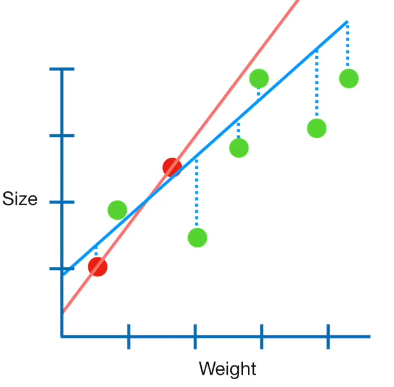
\includegraphics[scale=0.4]{figures/ridge.png}
	\end{figure}
\end{frame}


\begin{frame}{\textit{Ridge Regression}: Ventajas}
	\begin{itemize}
		\item Reduce la varianza.
		\pause
		\item Datos de Entrenamiento vs. Datos de Prueba.
		\pause
		\item Minimiza la influencia sobre el modelo de los predictores menos relacionados con la variable respuesta.
	\end{itemize}
\end{frame}

\begin{frame}{\textit{Ridge Regression}: Limitación}
	\begin{itemize}
		\item Modelo final incluye todos los predictores.
	\end{itemize}
\end{frame}

\begin{frame}{\textit{Lasso Regression}}
	\begin{itemize}
		\item Misma idea que en \textit{Ridge Regression}.
		\pause
		\item Realiza selección de predictores.
		\pause
		\item \textcolor{blue}{\textit{Shrinkage Penalty}} : $RSS_{\text{Lasso}} = RSS_{\text{AMC}} + \textcolor{blue}{\lambda \sum^p_{j=1} |\beta_j|}$.
	\end{itemize}
\end{frame}

\begin{frame}{Comparación entre \textit{Ridge} y \textit{Lasso Regression}}
	\begin{itemize}
		\item Usamos uno u otro dependiendo del escenario.
		\pause
		\item \textit{Ridge Regression}: cuando los $\B's \not = \mathbf{0}$ y tienen la misma magnitud aproximadamente.
		\pause
		\item \textit{Lasso Regression}: cuando un gran grupo de parámetros $\approx \mathbf{0}$.
	\end{itemize}
\end{frame}

\begin{frame}{Resultados de la implementación en R}
	\begin{itemize}
		\item Se usó el package \cod{glmnet}.
		\pause
		\item Se usó la misma fórmula que el modelo resultante con \textit{Backward} en \textit{Ridge} Regression.
		\pause
		\item En \textit{Lasso Regression} se consideró el modelo completo.
	\end{itemize}
\end{frame}

\begin{frame}{Resultados de la implementación en R}
	\begin{itemize}
		\item El $\lambda$ óptimo en los modelos nos dió:
		\pause
		\begin{itemize}
			\item \textit{Ridge Regression}: \textbf{0.05}.
			\item \textit{Lasso Regression}: \textbf{0.01}.
		\end{itemize}
		\pause
		\item Veamos algunos coeficientes importantes de los modelos.
	\end{itemize}
\end{frame}


\begin{frame}{Coeficientes de los modelos en orden creciente}
	\begin{center}
		\begin{tabular}{|r|c|c|c|}
			\hline
			Coeficiente & \textit{Backward}& \textit{Ridge} & \textit{Lasso} \\
			\hline
			Intercepto  &-48.2633 &-46.8465 &-44.4442 \\
			\cod{gmean\_ThermalConductivity} & -0.3338 & -0.3301 & -0.3171 \\
			\vdots & & & \\
			\cod{wtd\_range\_atomic\_radius} &  &  & 0\\
			\vdots & & & \\
			\cod{wtd\_entropy\_TConductivity}& 6.9492 & 6.7131 & 7.684503 \\
			\cod{Ba} & 9.3430 & 9.3538 & 10.6381 \\
			\hline
		\end{tabular}
	\end{center}
\end{frame}

\begin{frame}{Comparación entre modelos}
	\begin{itemize}
		\item La función que nos permite hacer \textit{Ridge} y \textit{Lasso Regression} no nos aporta información suficiente para calcular la \textit{Log-Verosimilitud}.
		\pause
		\item Un criterio de comparación es el $R^2$ ajustado:
		\pause
		\begin{itemize}
			\item \textit{Backward}: \textbf{0.66}.
			\item \textit{Ridge Regression}: \textbf{0.66}.
			\item \textit{Lasso Regression}: \textbf{0.65}.
		\end{itemize}
	\end{itemize}
\end{frame}

% RANDOM FOREST %%%%%%%%%%%%%%%%%%%%%%%%%%%%%%%%%%%%%%%%%%%%%%%%%%%%%%%%%%%%%%%%%%

\section{Extra}

\begin{frame}{\textit{Random Forest}}
	\begin{itemize}
		\item Árbol de decisión: \textit{Definición}.
		\pause
		\item Conjunto de estos árboles.
		\pause
		\item Boostrap.
		\pause
		\item Bootstrap.
		\pause
		\item Poco control sobre el modelo.
	\end{itemize}
\end{frame}

\begin{frame}{\textit{Random Forest}}
	\begin{figure}
		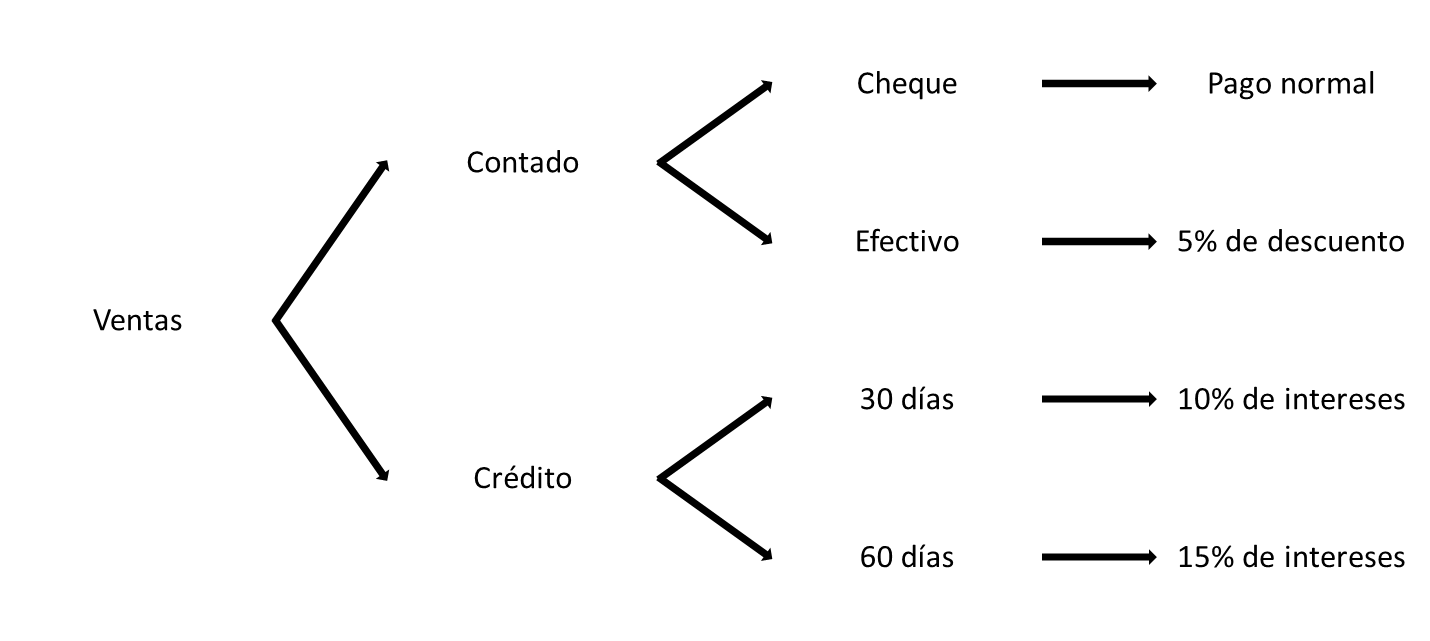
\includegraphics[scale=0.4]{figures/arbol-de-decisiones.png}
	\end{figure}
\end{frame}

\begin{frame}{\textit{Random Forest}: Implemantación}
	\begin{itemize}
		\item Package \cod{randomForest}.
		\pause
		\item El resultado es considerablemente mejor.
		\pause
		\item $R^2=\mathbf{0.92}$.
		\pause
		\item Veamos la gráfica de Valores Ajustados y Valores Reales:
	\end{itemize}
\end{frame}

\begin{frame}{\textit{Random Forest}: Densidad de Ajustados y Reales}

	\end{frame}

% CONCLUSIONES %%%%%%%%%%%%%%%%%%%%%%%%%%%%%%%%%%%%%%%%%%%%%%%%%%%%%%%%%%%%%%%%%%%%
\section{Conclusiones}

\begin{frame}{Conclusiones}
	\begin{itemize}
		\item Sobre los nuevos modelos.
		\pause
		\item Sobre el cumplimiento de los supuestos.
		\pause
		\item \textit{Random Forest}
		\pause
		\item \textit{Ridge} y \textit{Lasso Regression}.
		\pause
		\item Contraste con Avance \textbf{1}.
		\pause
		\item \textbf{¿Es suficiente una regresión múltiple?}
	\end{itemize}
\end{frame}


% REFERENCIAS %%%%%%%%%%%%%%%%%%%%%%%%%%%%%%%%%%%%%%%%%%%%%%%%%%%%%%%%%%%%%%%%%%%%%%%
\section{Referencias bibliográficas}

\begin{frame}{Referencias bibliográficas}
	\begin{thebibliography}{10}

		\beamertemplateonlinebibitems % imagen de una URL de internet
		\bibitem{Author2019}
		https://rpubs.com/Joaquin\_AR/255596
		\newblock{\em A.D., Random Forest ...}.
		\newblock{2017}

		\beamertemplateonlinebibitems % imagen de una URL de internet
		\bibitem{Author2019}
		https://rpubs.com/Joaquin\_AR/242707
		\newblock{\em Selección de predictores: Ridge y Lasso}.
		\newblock{2016}

		\beamertemplateonlinebibitems % imagen de una URL de internet
		\bibitem{Author2019}
		https://rstatisticsblog.com/data-science-in-action/machine-learning/ridge-regression-in-r/
		\newblock{\em Simple Guide To Ridge Regression In R}.
		\newblock{2020}

		%\beamertemplatebookbibitems % imagen de revista, paper o artículo
		%\bibitem{Author19901}
		%Libro
		%\newblock{\em Autor}.
		%\newblock{2020}

	\end{thebibliography}
\end{frame}


\end{document}

